\documentclass[xcolor=dvipsnames, compress]{beamer}
%\usetheme{Madrid} % My favorite!
\usetheme{Boadilla} % Pretty neat, soft color.
%\usetheme{Warsaw}
%\usecolortheme{dove} 
%\usetheme[secheader]{Boadilla}
% \useoutertheme[subsection=false]{smoothbars}
% \useinnertheme{rectangles}
% \usetheme{Marburg}
%   \usecolortheme[RGB={139,10,80}]{structure}
%  \usecolortheme[RGB={25,25,112}]{structure}
%\usecolortheme[RGB={255,127,36}]{structure}
%\usetheme{CambridgeUS}
%\usetheme{PaloAlto}
% \usefonttheme{professionalfonts}
% \usepackage{listings}

\usetheme{Boadilla}

% \usetheme{Warsaw}
%\usetheme{Darmstadt} %OK!
%  \usetheme{Frankfurt} %OK!
% \usetheme{Goettingen}
% \usetheme{Dresden}
%\usetheme{JuanLesPins} %OK!!
%\usetheme{Marburg}
%  \usetheme{Montpellier}
% \usetheme{Rochester} %sobrio
%\usetheme{Singapore}
%\usetheme{Szeged}
%\usetheme{Luebeck}

%\usetheme{Hannover}
%\usecolortheme{wolverine}

%\usecolortheme{albatross}
%\usecolortheme{seahorse}
%\usecolortheme{beetle}
%\usecolortheme{crane}
%\usecolortheme{dolphin}
%\usecolortheme{dove} %<- este con orchid
%\usecolortheme{fly}
%\usecolortheme{lily}
%\usecolortheme{orchid}
%\usecolortheme{rose}
%\usecolortheme{seagull}
%\usecolortheme{whale}

%\usetheme{Bergen} % This template has nagivation on the left
%\usetheme{Frankfurt} % Similar to the default 
%with an extra region at the top.
%\usecolortheme{seahorse} % Simple and clean template
%\usetheme{Darmstadt} % not so good
% Uncomment the following line if you want %
% page numbers and using Warsaw theme%
% \setbeamertemplate{footline}[page number]
%\setbeamercovered{transparent}
%\setbeamercovered{invisible}
% To remove the navigation symbols from 
% the bottom of slides%
%\setbeamertemplate{navigation symbols}{} 
%
\usepackage{graphicx}
\usepackage{amssymb,amsmath,amscd}
\usepackage{latexsym,xspace}
\usepackage[utf8]{inputenc}
\usepackage{epsfig}
%\usepackage{fancyhdr}
%\usepackage[spanish]{babel}
\usepackage[all]{xy}
\usepackage{enumerate}
\usepackage{eucal}
\usepackage[table, dvipsnames]{xcolor}
%\usepackage[usenames]{color}

\usepackage{mathtools} % flechas con nombres arriba o abajo

%#########################
\newcommand{\tx}{\ensuremath{\tau(X)}}
\newcommand{\txx}{\ensuremath{\tau_{X}}}
\newcommand{\Q}{\ensuremath{\mathbb{Q}}}
\newcommand{\Z}{\ensuremath{\mathbb{Z}}}
\newcommand{\N}{\ensuremath{\mathbb{N}}}
\newcommand{\R}{\ensuremath{\mathbb{R}}}
\newcommand{\C}{\ensuremath{\mathbb{C}}}
\newcommand{\A}{\ensuremath{\forall}}
\newcommand{\E}{\ensuremath{\exists}}
\newcommand{\iso}{\ensuremath{\cong}}
\newcommand{\union}{\ensuremath{\cup}}
%\newcommand{\morinyec}{\ensuremath{\precapprox}}
%\newenvironment{prueba}{\vspace{-3mm}\noindent\textbf{Demostraci\'on}\\}{\noindent$\blacksquare$\\}
\newcommand{\nin}{\ensuremath{\notin}}
\renewcommand{\emptyset}{\varnothing}

%\newcommand{\niso}{\ensuremath{\not \cong}}
\newtheorem{teor}{Teorema}[section]
\newtheorem{defi}{Definition}[section]
\newtheorem{ejemplo}{Examples}[section]
\newtheorem{obs}{Remark}[section]
\newtheorem{prop}{Proposition}[section]
\newtheorem{cor}{Corollary}[section]
\newtheorem{ntc}{Notation}[section]
\newtheorem{lema}{Lemma}[section]
\newtheorem{prob}{Problem}
\newtheorem{comen}{Comment}

%\usepackage{bm}         % For typesetting bold math (not \mathbold)
%\logo{\includegraphics[height=0.6cm]{yourlogo.eps}}
%
\title[Hidden Markov Chains]{Hidden Markov Chains}
\author{Marco, Nicolás, Sebastián and César}
\institute[ITAM]
%\date{November 7, 2019}
% \today will show current date. 
% Alternatively, you can specify a date.
%


\begin{document}
%
\begin{frame}
\titlepage
\end{frame}

\begin{frame}
\frametitle{Index}
 \tableofcontents%[sections]
\end{frame}

\begin{frame}
\section{Motivation }
\frametitle{Reminder: What a Markov chain is?}
\begin{itemize}	
	\item A Markov chain is a stochastic process with a particular characteristic, must be "memory-less" (i.e the probability of future actions are not dependent upon the steps that led up to the present state.). This property is known as the \textbf{Markov property}.
	\item Markov chains are very useful, we can find very often phenomena that satisfy the Markov property. This fact make Markov chains very useful in various application scenarios.
	\item Additionally, Markov chains allow us modelling sequential processes in a simple but effective way.	
\end{itemize}
\end{frame}

\begin{frame}
\section{Markov chains }
\frametitle{Reminder: What a Markov chain is?}
A simple example...
\begin{itemize}
	\item Bag of balls without replacement: \textbf{is NOT} a Markov process
	\begin{figure}
		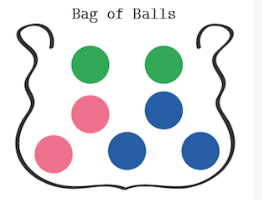
\includegraphics[scale=0.45]{ex1_bag_of_balls.png}
		\caption{example: probability of getting a blue ball / without replacement}
	\end{figure}
	\item Bag of balls with replacement \textbf{is} a Markov process
	\begin{figure}
		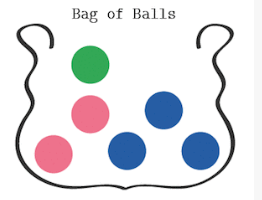
\includegraphics[scale=0.45]{ex1_bag_of_balls_wrep.png}
		\caption{example: probability of getting a blue ball / with replacement}
	\end{figure}
\end{itemize}
\end{frame}

\begin{frame}
\section{Markov Chains }	
\frametitle{Markov chains: Definition}
\begin{block}{Markov Chain: definition}
 A Markov chain is a sequence $X_{0:T}=\left(X_{0},X_{1},\ldots,X_{T}\right)$  of random variables taking values in some finite set $\mathcal{X}$ that satisfies the rule of conditional independence:
 \begin{equation*}
\mathds{P}\left(X_{t+1}=x_{t+1}\mid X_{t}=x_{t},\ldots,X_{0}=x_{0}\right)=\mathds{P}\left(X_{t+1}=x_{t+1}\mid X_{t}=x_{t}\right)
 \end{equation*}	
\end{block}
	
For this case, we will study time-homogeneous Markov chains (i.e. the probability of any state transition is independent of time).

\begin{equation*}
A_{i,j}:=\mathds{P}\left(X_{t+1}=j\mid X_{t}=i\right)\:i,j\in\mathcal{X}
\end{equation*}
		
However, the general case of Markov chains allows for time-inhomogeneous Markov chains (as time goes on, the probability of moving from one state to another may change). 	
\end{frame}


\begin{frame}
\frametitle{Transition matrices}
The movement among states are defined by a \textbf{transition matrix}, $A_{t}$. Particularly, this matrix contains the information on the probability of transitioning between states. 
\begin{equation*}
A_{i,j}:=\mathds{P}\left(X_{t+1}=j\mid X_{t}=i\right)\:i,j\in\mathcal{X}
\end{equation*}		
Each row of the matrix is a probability vector, and the sum of its entries is 1. 

For $x_{0}\in\mathcal{X}$, let $\mu_{x0}=\mathds{P}\left(X_{0}=x_{0}\right)$. Then, the joint promabiloty mass function of $X_{1:T}$ in terms of $\left(A_{i,j}\right)_{i,j\in\mathcal{X}}$ and $\left(\mu_{i}\right)_{i\in\mathcal{X}}$ is as follows: 

\begin{equation*}
p\left(x_{0:T}\right) & :=\mathds{P}\left(X_{0}=x_{0},\ldots,X_{T}=x_{t}\right)\\
& =\mathds{P}\left(X_{0}=x_{0}\right)\prod_{t=1}^{T}\mathds{P}\left(X_{t}=x_{t}\mid X_{t-1}=x_{t-1}\right)\\
& =\mu_{x0}\prod_{t=1}^{T}A_{x_{t-1},x_{t}}
\end{equation*}		
\end{frame}

\begin{frame}
\section{Hidden Markov Chains }
\frametitle{Hidden Markov Chains : Motivation}
\begin{itemize}
	\item A  \textbf{Hidden Markov Model} is a statistical model which studies a system assumed as a Markov process including hidden (unobservable) states. 
	\item In the simple Markov chain model, the state of the system is directly visible to the observer. On the other hand, HMM assume that the data observed is not the actual state of the model but instead is generated by underlying hidden states.
	\item Each state has a probability distribution over the possible outputs. 
	\item HMM are often used to model temporal data.
\end{itemize}
\end{frame}

\begin{frame}
\frametitle{Definition}
\begin{block}{HMM :Definition}
	Let $X_{0:T}=\left(X_{0},X_{1},\ldots,X_{T}\right)$ be a homogeneous Markov chain taking values in $\mathcal{X}$ with and associated transition matrix $\left(A_{ij}\right)$. Additionally, there exits another sequence of random variables $Y_{0:T}=\left(Y_{1},\ldots,Y_{T}\right)$ taking values in $\mathcal{Y}$, known as the observation space. 
\end{block}	

We assume that the random variables of sequence $Y_{0:T}$ are independent conditional on the state sequence $X_{0:T}$, which is equivalent to:
\begin{equation*}
\mathds{P}\left(Y_{1}=y_{1},\ldots,Y_{T}=y_{T}\mid X_{0}=x_{0},\ldots,X_{T}=x_{t}\right)=\prod_{t=1}^{T}\mathds{P}\left(Y_{t}=y_{t}\mid X_{t}=x_{t}\right)
\end{equation*}	
	
if we are considering an homogeneous HMM, then we have an  \textbf{emission probability} mass function:
\begin{equation*}
g_{x}(y):=\mathds{P}\left(Y_{t}=y\mid X_{t}=x\right)
\end{equation*}	
\end{frame}

\begin{frame}
\frametitle{More Definitions}
Using the emission probabilities to connect the observation space and the hidden space and introducing the transition matrix that governs the movements among hidden states, we can define the  joint probability of the hidden states and observations as follows:
\begin{equation*}
\mathds{P}\left(X_{0:T}=x_{0:T},Y_{0:T}=y_{0:T}\right)=\mu_{x_{0}}\prod_{t=1}^{T}g_{x_{t}}\left(y_{t}\right)A_{x_{t-1},x_{t}}
\end{equation*}	
\end{frame}

% Marco Diap 11
\begin{frame}
\frametitle{Example}
Where is the frog at the beginning?
\begin{center}
	\begin{table}
		\begin{centering}
			\begin{tabular}{|c|c|c|c|c|c|}
				\hline 
				\rowcolor{lightgray}
				1 & 2 & 3 & 4 & 5 & 6\tabularnewline
				\hline 
				\hline 
				1/6 & 1/6 & 1/6 & 1/6 & 1/6 & 1/6\tabularnewline
				\hline 
			\end{tabular}
			\par\end{centering}
		\caption{Hidden Mark-frog chain example - Part I}
	\end{table}
	\par\end{center}
\end{frame}

% Marco Diap 12
\begin{frame}
\frametitle{Example - Transition probabilities (Matrix A)}
Where can the frog jump? 

\begin{center}
	\begin{table}
		\begin{centering}
			Level to
			\par\end{centering}
		\begin{centering}
			Level from%
			\begin{tabular}{|c|c|c|c|c|c|c|}
				\hline 
				\rowcolor{lightgray}
				& 1 & 2 & 3 & 4 & 5 & 6\tabularnewline
				\hline 
				\hline 
				1 & 0.4 & 0.6 &  &  &  & \tabularnewline
				\hline 
				2 & 0.3 & 0.4 & 0.6 &  &  & \tabularnewline
				\hline 
				3 &  & 0.3 & 0.4 & 0.6 &  & \tabularnewline
				\hline 
				4 &  &  & 0.3 & 0.4 & 0.6 & \tabularnewline
				\hline 
				5 &  &  &  & 0.3 & 0.4 & 0.6\tabularnewline
				\hline 
				6 & 0.6 &  &  &  & 0.3 & 0.4\tabularnewline
				\hline 
			\end{tabular}
			\par\end{centering}
		\caption{Hidden Mark-frog chain example - Part II}
		
	\end{table}
	\par\end{center}
\end{frame}

% Marco diap 13
\begin{frame}
\frametitle{Example - Emission probabilities (Matrix B)}
What is the probability to detect the frog?

	\begin{center}
	
\includegraphics[width=0.2\textwidth]{images/sensor.png}
	\end{center}

\begin{center}
	\begin{table}
		\begin{centering}
			\begin{tabular}{|c|c|c|}
				\hline 
				& Detection & No detection\tabularnewline
				\hline 
				\hline 
				1 & 0.9 & 0.1\tabularnewline
				\hline 
				2 & 0.5 & 0.5\tabularnewline
				\hline 
				3 & 0.1 & 0.9\tabularnewline
				\hline 
				4 & 0 & 1\tabularnewline
				\hline 
				5 & 0 & 1\tabularnewline
				\hline 
				6 & 0 & 1\tabularnewline
				\hline 
			\end{tabular}
			\par\end{centering}
		\caption{Hidden Mark-frog chain example - Part III}
	\end{table}
	\par\end{center}
\end{frame}

% Marco diap 14
\begin{frame}
\frametitle{Example - Observations}
After 14 times, this are the sensor\textquoteright s results: 
\begin{center}
	\begin{table}
		\begin{centering}
			\begin{tabular}{|c|c|c|c|c|c|c|c|c|c|c|c|c|c|}
				\hline 
				1 & 2 & 3 & 4 & 5 & 6 & 7 & 8 & 9 & 10 & 11 & 12 & 13 & 14\tabularnewline
				\hline 
				\hline 
				0 & 0 & 0 & 0 & 1 & 1 & 0 & 0 & 0 & 0 & 1 & 1 & 0 & 1\tabularnewline
				\hline 
			\end{tabular}
			\par\end{centering}
		\caption{Hidden Mark-frog chain example - Part IV}
	\end{table}
	\par\end{center}
\end{frame}

% Marco diap 15
\begin{frame}
\frametitle{Using filtering algorithm}
\textbf{Forward Algorithm initialization equation}
$$ \alpha_{1}(i) = \pi_i \cdot b_{i}(O) $$
	
\textbf{Forward Algorithm recursion equation}
$$ \alpha_{t+1}(j) = \sum_{i=1}^N \alpha_t(i) \alpha_{ij} b_{ij}(O) $$
	
\textbf{Termination}
$$ P(O|\lambda) = \sum_{i=1}^N \alpha_T(i)$$
\end{frame}

% Marco diap 16
\begin{frame}
\frametitle{Distribution of X (filtering)}
	\begin{center}
	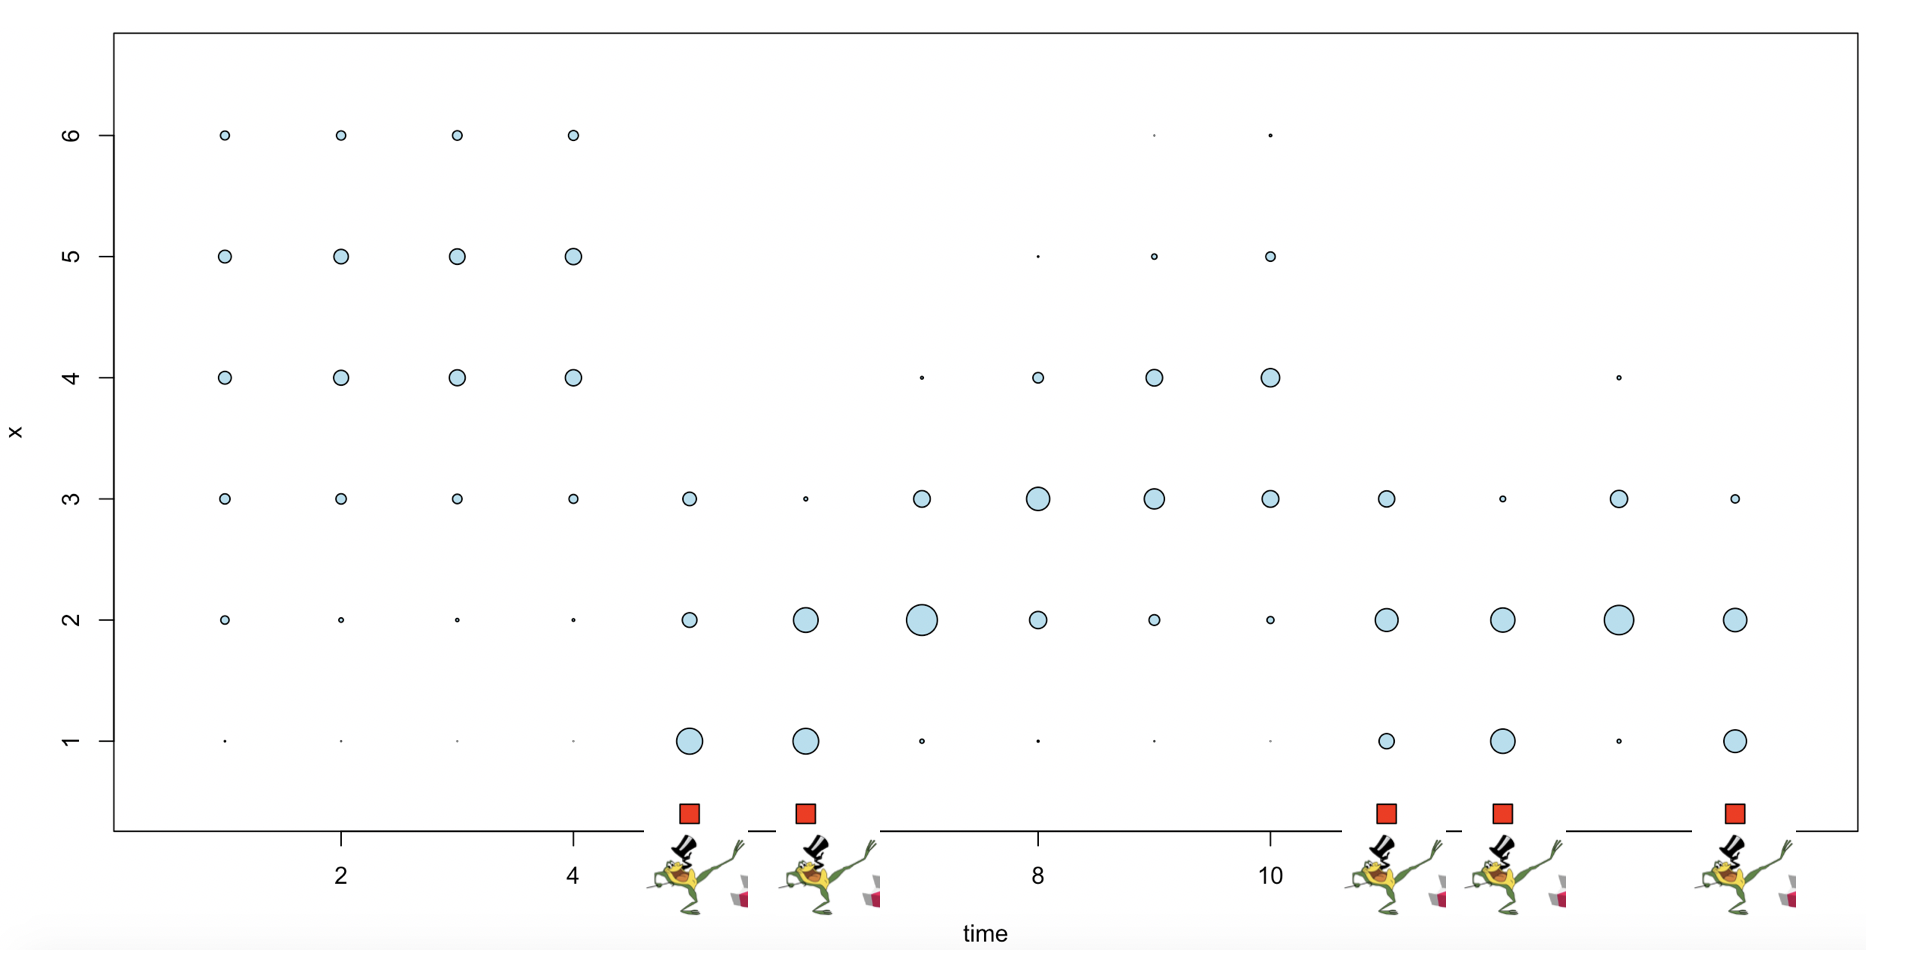
\includegraphics[width=0.7\textwidth]{images/ex_filtering_marco.png}
\end{center}
\end{frame}

% Marco diap 17
\begin{frame}
\frametitle{Distribution of $X$ (smoothing)}
	\begin{center}
	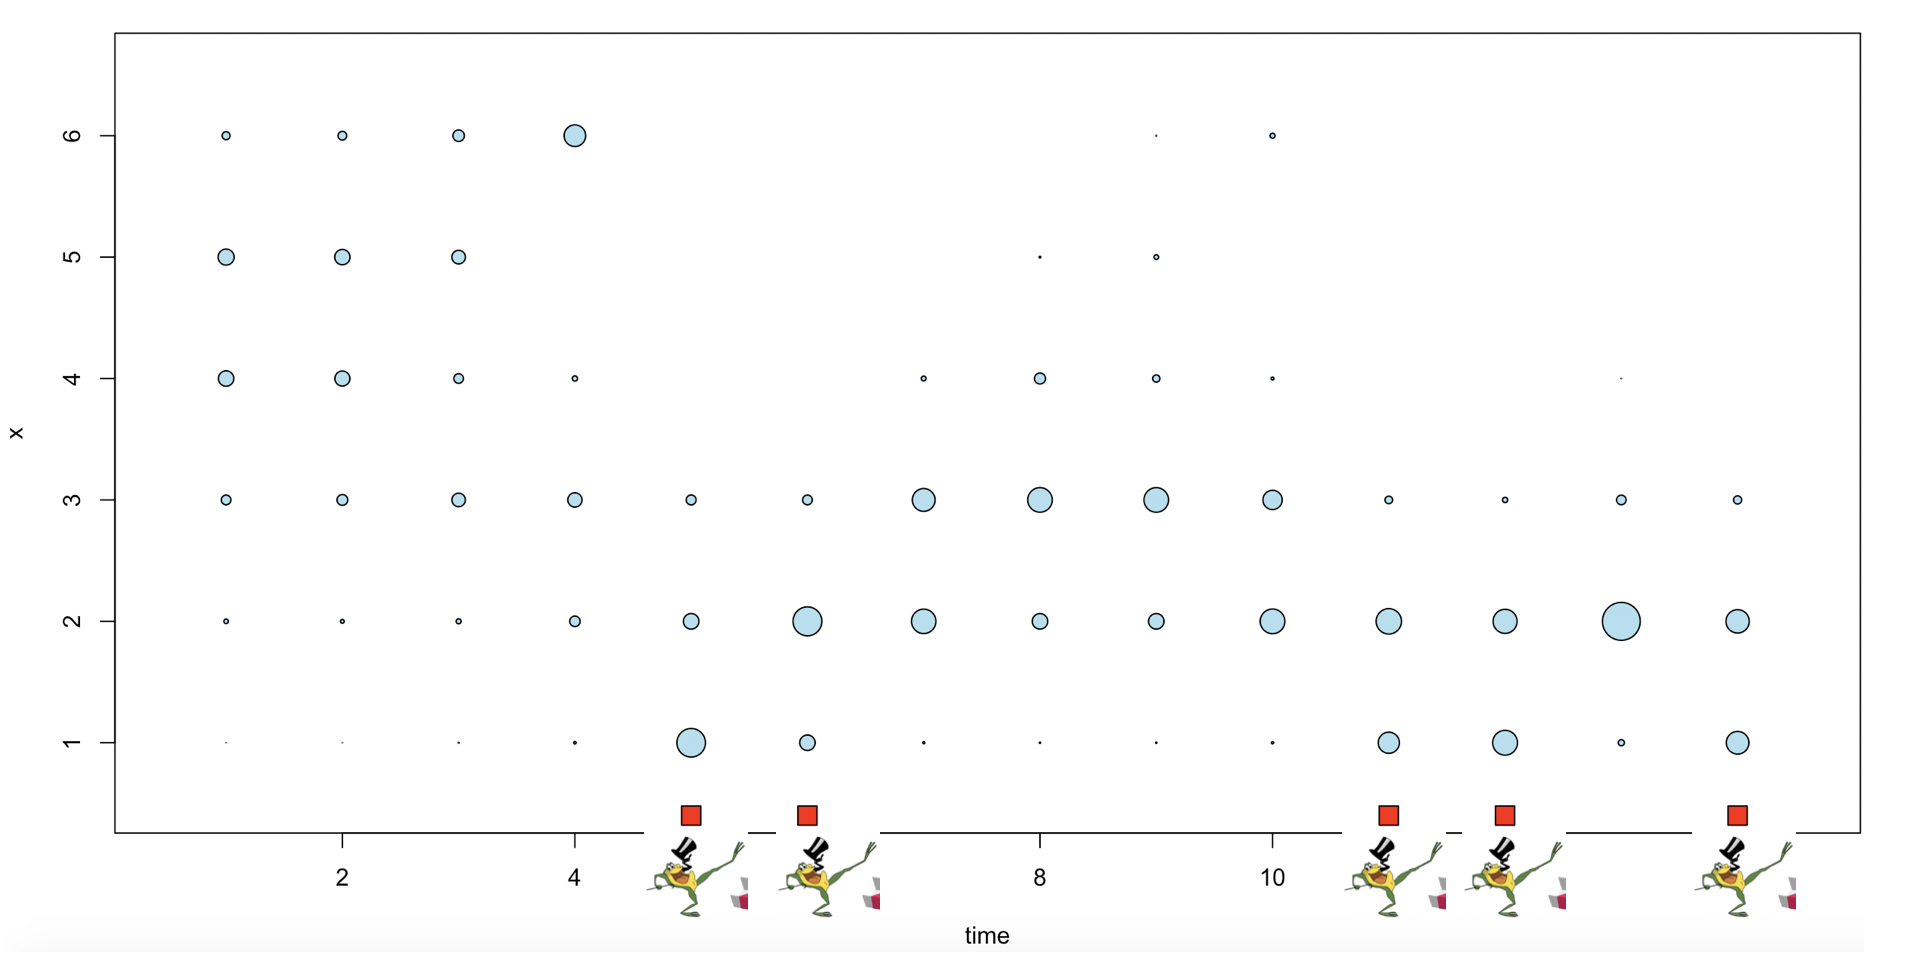
\includegraphics[width=0.7\textwidth]{images/ex_smoothing_marco.png}
\end{center}
\end{frame}

% Marco diap 18
\begin{frame}
\frametitle{Decoding of X}
\begin{center}
	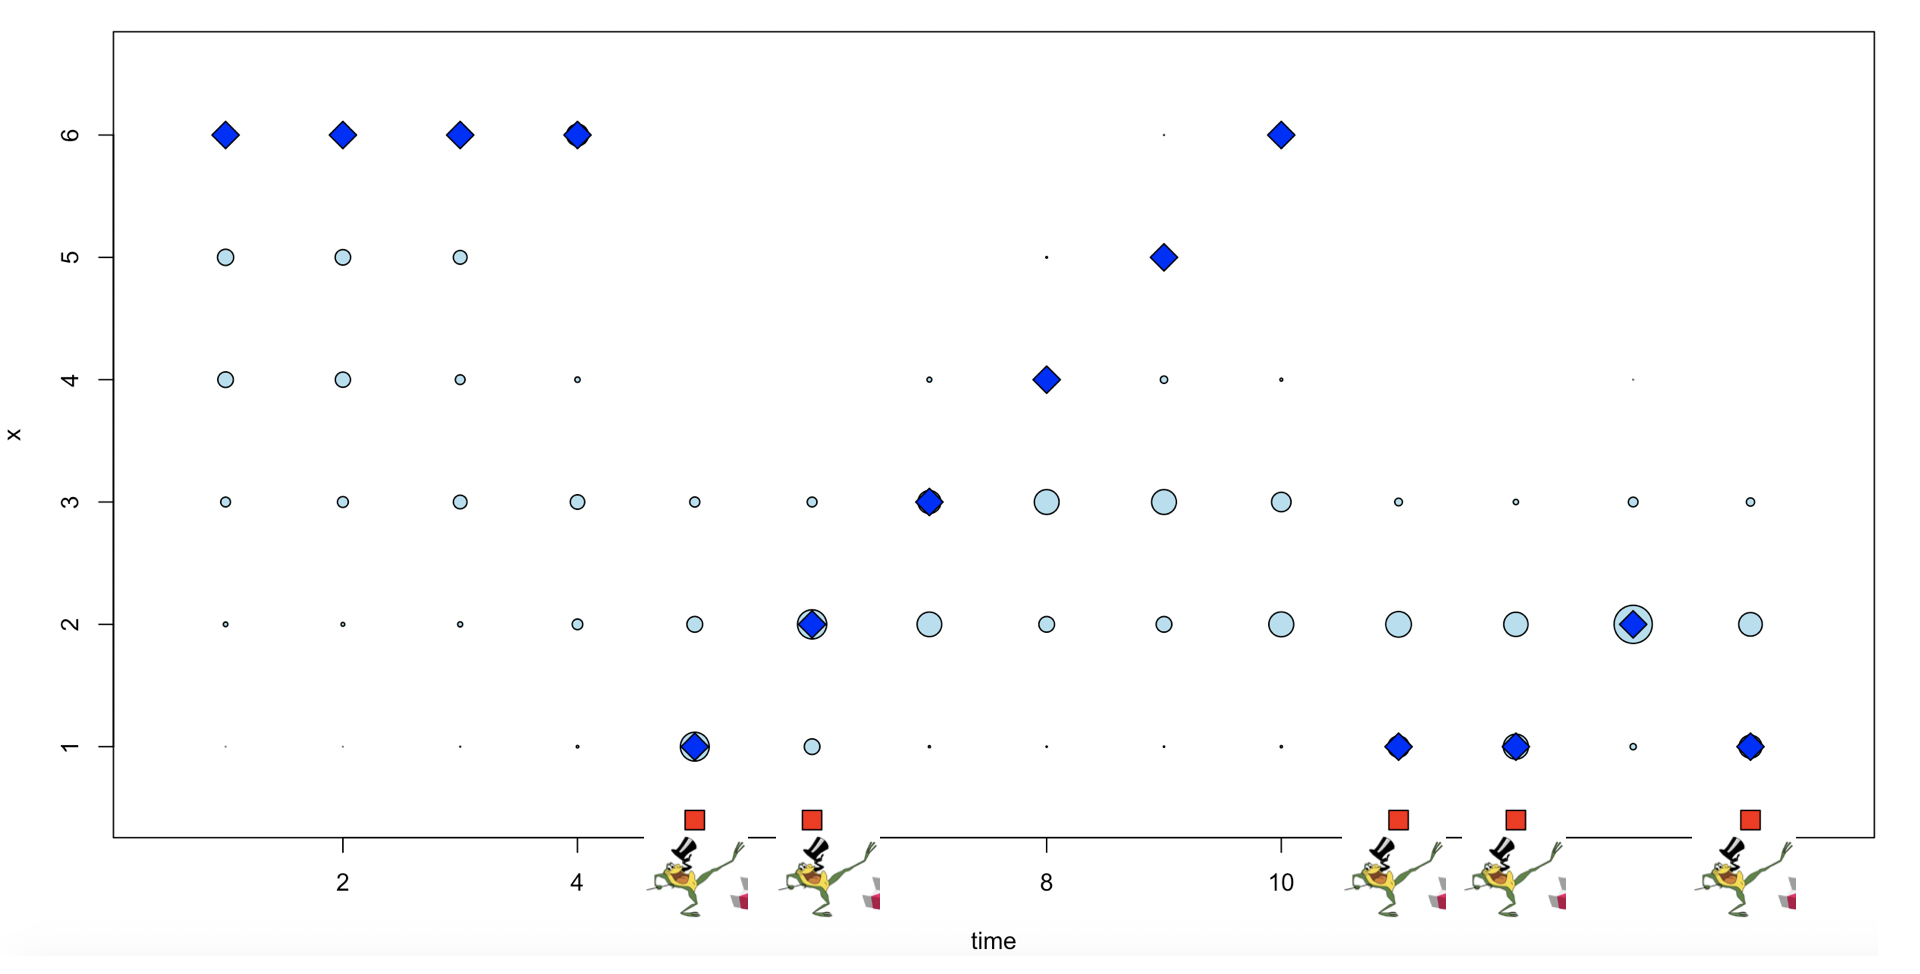
\includegraphics[width=0.7\textwidth]{images/ex_decoding_marco.png}
\end{center}
\end{frame}

% Marco diap 19
\begin{frame}
\frametitle{Formal Filtering}
We are interested in the conditional probability mass function $p\left(x_{t}\mid y_{1:t}\right)$ of the state $X_{t}$ given the data observed up to time $t$ .

$$ p(x_t|y_{1:t}) = \frac{p(x_t, y_{1:t})}{ \sum_{x_t^\prime \in \mathcal{X}} p(x_t^\prime, y_{1:t}) }$$

\end{frame}

\begin{frame}
\frametitle{Formal Filtering}
We will derive a recursion for:
\hspace{-0.2cm}
\begin{eqnarray*}
\textcolor{red}{p(x_t,y_{t	:T})} & = & \sum_{x_{t-1} \in \mathcal{X}} p(x_t, x_{t-1}, y_t, y_{1:t-1})\\
& = & \sum_{x_t \in \mathcal{X}} p(y_{t}| x_t, x_{t-1}, y_{1:t-1} ) p(x_{t} |x_{t-1},y_{1:t-1}) p(x_{t-1},y_{1:t-1}) \\
& = &  p(y_{t}|x_t) \sum_{x_t \in \mathcal{X}} p(x_{t}|x_{t-1}) \textcolor{red}{ p(x_{t-1},y_{1:t-1})}   
\end{eqnarray*}

If we define $\alpha(t):= p(x_{t},y_{1:t})$, then we have a forward recursion for $t=1, \ldots, T$, $x_t\in \mathcal{X}$:
$$ \textcolor{red}{\alpha_{t}(x_{t})} = p(y_{t}|x_t) \sum_{x_t \in \mathcal{X}} p(x_{t}|x_{t-1}) \textcolor{red}{\alpha_{t-1}(x_{t-1})}; \mbox{ } \alpha_0(x_0)=0 $$
\end{frame}

% Marco diap 20
\begin{frame}
\frametitle{Formal Filtering and likelihood}
So, we compute a filtering using: 

For $t=1,\ldots,T$, $x\in X$:

\[
\alpha_{t}\left(x_{t}\right)=p\left(y_{t}\mid x_{t}\right)\sum_{x_{t-1}\in\mathcal{{X}}}p\left(x_{t}\mid x_{t-1}\right)\alpha_{t-1}\left(x_{t-1}\right)
\]	
\end{frame}

\begin{frame}
\frametitle{Formal Filtering and likelihood}

The filtering pmf is obtained by normalizing $\alpha_{t}\left(x_{t}\right)$
as: 
$$p(x_t| y_{1:t}) = \frac{p(x_t, y_{1:t})}{p(y_{1:t})}  = \frac{\alpha_t(x_t)}{ \sum_{x \in \mathcal{X}} \alpha_t(x) }$$
The likelihood term $p\left(y_{1:t-1}\right)$ can be computed from
the $\alpha$-recursion:
$$p(y_{1:T}) =  \sum_{x \in \mathcal{X}} \alpha_T(x) $$
\textbf{Predict}
$$p(x_t| y_{1:t-1}) = \sum_{x_{t-1} \in \mathcal{X}} p(x_t|x_{t-1}) p(x_{t-1}|y_{1:t-1}) $$
\textbf{Update}
$$p(x_t| y_{1:t}) = \frac{g_{x_t}(y_t) p(x_t|y_{1:t})}{\sum_{x_{t}^\prime \in \mathcal{X}} g_{x_t^\prime}(y_t) p(x_t^\prime|y_{1:t})} $$
\end{frame}

% Marco diap 21
\begin{frame}
\frametitle{Considerations in Filtering}
\begin{itemize}
	\item 	The proposed recursion may suffer from numerical underflow/overflow,
	as $\alpha_{t}$ may become very small or very large for large $t$. 
	\item  The proposed recursion may suffer from numerical underflow/overflow,
	as $\alpha_{t}$ may become very small or very large for large $t$. 
	\item To avoid this, we can normalize $\alpha_{t}$, or propagate the filtering
	\emph{pmf $p\left(x_{t}\mid y_{1:t}\right)$ }instead of $\alpha_{t}$,
	using the following two-step predict-update recursion:
\end{itemize}
$$
p\left(x_{t}\mid y_{1:t-1}\right)=\sum_{x_{t-1}\in\mathcal{{X}}}p\left(x_{t}\mid x_{t-1}\right)p\left(x_{t-1}\mid y_{1:t-1}\right)\qquad Predict
$$

$$
p\left(x_{t}\mid y_{1:t}\right)=\frac{g_{x_{t}}\left(y_{t}\right)p\left(x_{t}\mid y_{1:t-1}\right)}{\sum_{x_{t}^{'}\in\mathcal{{X}}}g_{x'_{t}}\left(y_{t}\right)p\left(x'_{t}\mid y_{1:t-1}\right)}\qquad Update
$$
\end{frame}



%
%\begin{frame}[fragile] % Notice the [fragile] option %
%\frametitle{Verbatim}
%\begin{example}[Putting Verbatim]
%\begin{verbatim}
%\begin{frame}
%\frametitle{Outline}
%\begin{block}
%{Why Beamer?}
%Does anybody need an introduction to Beamer?
%I don't think so.
%\end{block}
% Extra carriage return causes problem with verbatim %
%\end{frame}\end{verbatim} 
%\end{example}
%\end{frame}
 
%\begin{frame}[fragile]  % notice the fragile option, since the body
			% contains a verbatim command
%Example of the \verb|\cite| command to give a reference is below:
%Example of citation using \cite{key1} follows on.
%\end{frame}
 
% \begin{frame}
% \section{Bibliografía}
% \frametitle{Referencias}
% \footnotesize{
% \begin{thebibliography}{99}
%  \bibitem[Morita, 2010]{key1} J. Nagata, K. Morita (1989)
%  \newblock Topics On General Topology.
%  \newblock \emph{Elsevier Science Publisher B.V.} 15(6), 203 -- 243.

% \bibitem[VanMill, 2010]{key1} J. Van Mill ; M. Husek (1992)
%  \newblock Recent Progress In General Topology.
%  \newblock \emph{Elsevier Publications} p. 375.

% \bibitem[MacLane, 2010]{key1} J. S. Mac Lane(1971)
%  \newblock Categories for the working mathematician,.
%  \newblock \emph{Springer} p. 375.

%  \bibitem[Ishii, 2010]{key1} Tadashi Ishii (1969)
%  \newblock On Tychonoff Functor and $w$-Compactness.
%  \newblock \emph{Topology Appl.} 11, 175 -- 187.

%  \bibitem[Ishii, 2010]{key1} T. Hoshina; K. Morita (1980)
%  \newblock On Regular Products Of Topological Spaces.
%  \newblock \emph{Topology Appl.} 11, 47 -- 57.
% \end{thebibliography}
% }
% \end{frame}


 
% \begin{frame}
% %\section{Bibliografía}
% \frametitle{Referencias}
% \footnotesize{
% \begin{thebibliography}{99}
%  \bibitem[Porter, 2010]{key1}J. R. Porter ; R. Grant Woods  (1987)
%  \newblock Extensions and Absolutes of Hausdorff Spaces.
%  \newblock \emph{Springer-Verlag} 856.


%  \bibitem[Simon, 2010]{key1} Petr Simon (1984)
%  \newblock Completely regular modification and products.
%  \newblock \emph{Commentationes Mathematicae Universitatis Carolinae} 25(1), 121--128.



%  \bibitem[Puppier, 2010]{key1} René Puppier (1969)
%  \newblock La Completion Universelle D'un Produit D'espaces Completement Reguliers .
%  \newblock \emph{Publ. Dept. Math, Lyon} 254, 342--351.



% \end{thebibliography}
% }
% \end{frame}
% 
% End of slides
\end{document} 